\documentclass[english, a4paper, 12pt, twoside]{insea} 

% based on the NHH master template thesis template made by Endre Bjørndal

\date{2024 - 2025}
\title{Optimization of Multi Agent Collaboration for Dynamic Target Acquisition}
\author{M. Boulaich Mohamed}
\supervisor{Mme. Btissam El KHAMLICHI && M. Hicham JANATI}

\graphicspath{{Images/}{../Images/}}
\setbib{References}
  

% ----- Document starts here ----- 
\begin{document}


\def\biblio{} % resets the biblio command, if not here a new reference list will be produced after every chapter

% 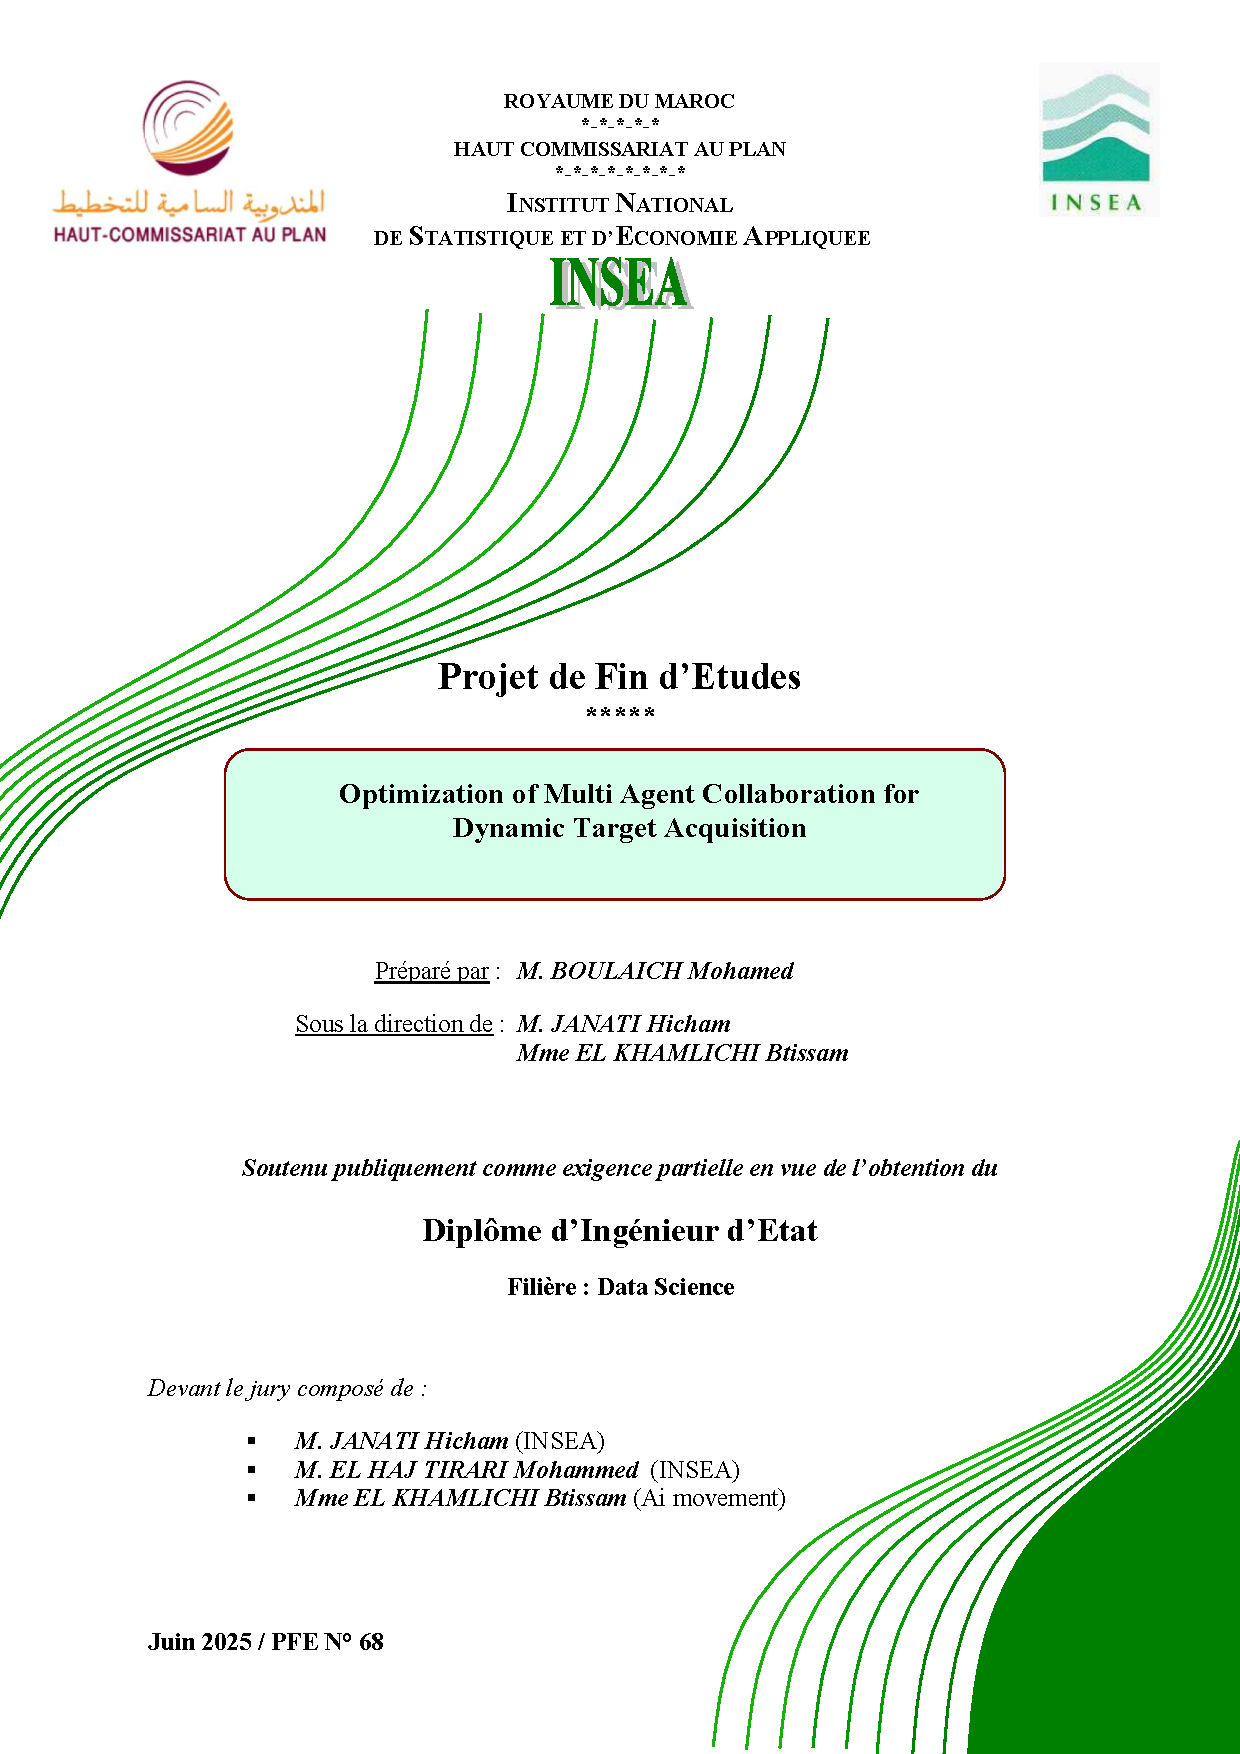
\includepdf[pages=1]{cover-page.pdf}
\maketitle

\restoregeometry % restores the margins after frontpage
%\nocite{*} % uncomment if you want all sources to be printed in the reference list, including the ones which are not cited in the text 

\pagenumbering{gobble} % suppress page numbering
\thispagestyle{plain} % suppress header
\clearpage\mbox{}\clearpage % add blank page

\pagenumbering{roman} % starting roman page numbering
\newpage
    \subfile{Chapters/Acknowledgements}

\newpage
\chapter*{Abstract}
    \addcontentsline{toc}{chapter}{Abstract} % Adds this page to the Table of Contents
    \subfile{Chapters/Abstract}

\newpage
\chapter*{Résumé}
    \addcontentsline{toc}{chapter}{Résumé} % Adds this page to the Table of Contents
    \subfile{Chapters/Resume}

\newpage
\tableofcontents
\listoffigures
\listoftables

\chapter*{List of Acronyms}
    \addcontentsline{toc}{chapter}{Acronyms} % Adds this page to the Table of Contents
    \subfile{Chapters/Acronyms}
\clearpage



\newpage

\pagenumbering{arabic} % Starting arabic page numbering
\setcounter{page}{1} % sets pagecounter to 1


\chapter*{General Introduction}
    \addcontentsline{toc}{chapter}{General Introduction} % Adds this page to the Table of Contents
    \subfile{Chapters/01-Introduction}
\clearpage

\chapter{General Project Context}
    \subfile{Chapters/02-Context}
\clearpage

\chapter{Theoretical Foundations of the Project}
    \subfile{Chapters/03-1-Theory-rl-foundation}
    \subfile{Chapters/03-2-Theory-rl-algo}
    \subfile{Chapters/03-3-Theory-marl-qmix}
\clearpage

\chapter{Experimental Methodology and Results}
    \subfile{Chapters/04-1-Project-setup}
    \subfile{Chapters/04-2-Project-intuition}
    \subfile{Chapters/04-3-Project-experiment}
\clearpage

\chapter*{Conclusion and Future Work}
    \label{chap:conclusion}
    \addcontentsline{toc}{chapter}{Conclusion and Future Work} % Adds this page to the Table of Contents
    \subfile{Chapters/05-Conclusion}
\clearpage

\newpage
% \renewcommand\refname{References} % name for the reference list
\renewcommand\bibname{References} % Use References as the title of the bibliography chapter

{\setstretch{1.0} % linespacing for the references
\addcontentsline{toc}{chapter}{\refname} % to change the name of the references in the TOC
\bibliography{References.bib} % adds the references to the document
}


\newpage
\renewcommand{\appendixpagename}{Annexe} % Heading of appendix
\renewcommand{\appendixtocname}{Annexe} % name of appendix in TOC
%\appendixpage 
\addappheadtotoc


% \begin{appendices}
%     \subfile{Chapters/Appendix}
% \end{appendices}


% TIPS AND TRICKS - REMOVE WHEN YOU DON'T NEED IT ANYMORE
% \newpage
% \section{Tips and tricks to get you started}
%     \subfile{Chapters/Tips}

\end{document}
